\chapter{Wprowadzenie}

Widzenie maszynowe jest jedną z~najprężniej rozwijających się
dziedzin z~pogranicza algorytmiki, optymalizacji, przetwarzania obrazów,
przetwarzania sygnałów, statystyki oraz szeroko pojętej sztucznej
inteligencji jeżeli chodzi o~zagadnienia informatyczne w~ostatnich
latach. Sporządzenie definicji widzenia komputerowego jest niezmiernie
trudne, głównie z~powodu wspomnianej interdyscyplinarności, 
jaką niesie ze sobą omawiany termin. Klasyczne, jednozdaniowe
definicje przedstawiają w~zwięzły sposób ogólny zarys koncepcji,
jaka kryje się za sformułowaniami określanymi mianem wizji komputerowej.
Wysoki poziom abstrakcji oraz zwięzłość formy zmuszają do pominięcia
wielu istotnych aspektów, które nienaświetlone mogą w~poważny sposób
zaburzyć wyobrażenie o~tymże jak niezmiernie interesującym 
obszarze nauki i~techniki.  
Poniżej przedstawiono kilka definicji wprowadzonych na przestrzeni
kilkunastu ostatnich lat. 

DEFINICJA 1 \cite{ShapiroStockman200102}:

\blockquote{Zadaniem wizji komputerowej jest podejmowanie 
decyzji na temat rzeczywistych (fizycznych) obiektów
oraz scen na podstawie obrazów.}

W~komentarzu do zaprezentowanej definicji wprowadzony został
cel pośredni. Aby podjęcie decyzji na temat rzeczywistych obiektów
było możliwe, niemal zawsze niezbędne jest sporządzenie ich modelu lub 
opisu na podstawie posiadanych zdjęć. Zgodnie z~powyższym 
równolegle do poprzedniej definicji, zaproponowana została druga, mniej
abstrakcyjną wersja, którą umieszczono poniżej.

DEFINICJA 2 \cite{ShapiroStockman200102}:

\blockquote{Zadaniem wizji komputerowej jest sporządzanie
opisów scen rzeczywistych na podstawie obrazów.}

Jest to pierwsza próba ograniczenia danych wyjściowych jakich należałoby
oczekiwać po uruchomieniu procesu określanego mianem wizji komputerowej.

Następna definicja jest kolejną próbą
podjętą w~kierunku maksymalnego uproszczenia i~zawężenia
przeciwdziedziny widzenia komputerowego. Nie ulega raczej wątpliwości,
że danymi wejściowymi procesu są obrazy lub sekwencje obrazów.
W~tym kontekście następne zdanie definiuje produkt omawianego zagadnienia.

DEFINICJA 3 (na podstawie \cite{morris2004computer}):

\blockquote{Wizja komputerowa obejmuje swym zakresem wydobywanie
danych numerycznych z~obrazów.}

Tak jak przetwarzanie obrazów określa działania na obrazach wynikiem
których są obrazy o~zmienionych właściwościach w~porównaniu do obrazów
wejściowych, tak wynikiem widzenia komputerowego są dane wydobywane
z~obrazów. Dane wyłuskane w~ten sposób mogą zostać wykorzystane
na wiele sposobów:
\begin{itemize}
    \item prezentując wartość samą w~sobie, np.: odczyt tekstu
        z~zeskanowanych dokumentów (OCR),
    \item określając współrzędne elementów sceny, w~kontekście OCR 
        i~odczytywania tekstu z~dokumentów dane tego typu
        wykorzystywane są do zachowania struktury dokumentu, tabel,
        obrazów itp.
    \item do uwierzytelniania na podstawie danych biometrycznych - 
        rozpoznawanie i~identyfikacja siatkówki oka,
    \item do budowania modeli trójwymiarowych obiektów na podstawie 
        sekwencji obrazów, itp.
\end{itemize}

Jak łatwo zauważyć widzenie komputerowe to niezwykle pojemny termin.
Interdyscyplinarność czyni próbę wymienienia zagadnień z~nim związanych,
bez pominięcia jakiejś istotnej gałęzi, niemal niemożliwą. 
Złożoność i~rozległość zakresu jaki wiąże się
z~tym zagadnieniem zilustrowano na rys. \ref{fig:int_cv_inter_discip}.

\begin{figure}[!h]
    \centering
    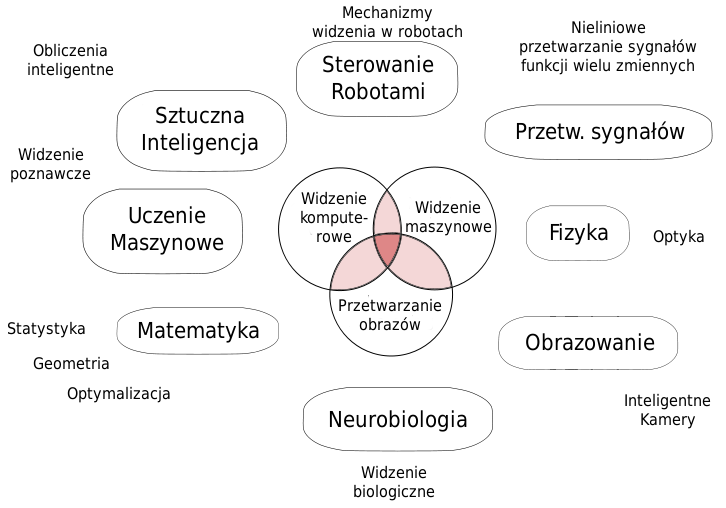
\includegraphics[width=0.9\textwidth]{img/int_cv_inter_discip}
    \caption{Powiązanie wizji komputerowej z~innymi dziedzinami 
        (na podstawie \cite{wiki:computervision})}
    \label{fig:int_cv_inter_discip}
\end{figure}

Za początek widzenia maszynowego, w~bardzo dużym przybliżeniu, można
uznać początek drugiej połowy ubiegłego wieku.
W~latach pięćdziesiątych wdrożone zostały dwie implementacje 
pierwszego komercyjnego systemu OCR (\textit{ang. Optical Character 
Recognition}). Pierwszym klientem było wydawnictwo Reader's Digest, 
gdzie system wykorzystywano do automatycznego odczytywania adresów
z~przesyłek wysyłanych do czytelników w~celu ich sortowania.
Drugim klientem komercyjnego systemu OCR 
była firma Standard Oil Company. Rozwiązanie
służyło odczytywaniu danych z~kart kredytowych w~celach 
rozliczeniowych \cite{WEB:ocrhistory}.

Obecnie istnieje wiele narzędzi do odczytywania tekstu z~zeskanowanych
dokumentów, przy czym najlepsze rozwiązanie dostępne na rynku
można nabyć za cenę niewiele wyższą od tej w~jakiej oferowany jest
popularny pakiet oprogramowania biurowego.

Według innego opracowania \cite{web:huangcvevolution}
początki widzenia komputerowego są związane z~nazwiskiem Larrego
Robertsa. On to przez swoją pracę doktorską na temat możliwości
wyłuskania trójwymiarowych współrzędnych brył geometrycznych
z~dwuwymiarowych widoków perspektywicznych został okrzyknięty
,,ojcem'' wizji komputerowej. Praca została złożona i~obroniona 
w~latach 60 na uczelni MIT \cite{books/garland/Roberts63}.

Ważnym wydarzeniem z~perspektywy niniejszej pracy dyplomowej była
implementacja algorytmu wykrywającego wystąpienie twarzy
w~obrazie w~czasie rzeczywistym.
Na początku obecnego stulecia opracowano oraz zaimplementowano algorytm
\cite{DBLP:conf/cvpr/ViolaJ01}, który uruchomiony na komputerze 
z~procesorem Intel Pentium III 700 MHz był wstanie przeszukać 15 
obrazów na sekundę pod kątem wystąpienia twarzy.
Rozdzielczość obrazów wejściowych była równa 384 na 288 pikseli.
Dzisiaj, ze względu na moc obliczeniową urządzeń mobilnych, algorytm ten 
bez trudu można uruchomić
na telefonie lub aparacie fotograficznym. 
Ponadto uzyskane wyniki przekraczają wspomniane 15 obrazów na sekundę
przy jednoczesnym wykorzystaniu obrazów wejściowych w~znacznie
większej rozdzielczości: 720p czy nawet 1080p.
Jedną z~bardziej 
popularnych funkcjonalności opartych na wspomnianym rozwiązaniu 
jest wykorzystywany od kilku lat system zwalniania migawki w~aparatach
cyfrowych.
Zdjęcie wykonywane jest
po wykryciu twarzy w~kadrze zawierającej określony grymas, na przykład
uśmiech.

Moc obliczeniowa współczesnych smartfonów pozwala na uruchomienie
znacznie bardziej skomplikowanych algorytmów. Najnowsze jednostki,
wyposażone w~procesory cztero i ośmiordzeniowe można nabyć
w~cenie już kilkuset złotych. Dodatkowo mnogość dostępnych bibliotek 
sprawia, że głównym ograniczeniem przy projektowaniu i~implementacji
rozwiązań z~dziedziny widzenia komputerowego jest już niemal
tylko wyobraźnia. Co prawda, utrudnieniem może być słabej jakości
kamera dostępna w~urządzeniu, jednak ograniczenie to obowiązuje
tylko podczas implementacji algorytmów precyzyjnej lokalizacji
i~rozpoznawania obiektów na podstawie danych z~aparatu.

Jednym z~popularniejszych zastosowaniem widzenia komputerowego w~telefonach
jest odczytywanie kodów QR. Jest to często stosowana technika
np. w~muzeach. Aplikacje udostępniane przez placówki 
umożliwiają uzyskanie szczegółowych opisów eksponatów na
podstawie zamieszczonych obok nich kodów. Zwiedzający mogą w~ten sposób 
skorzystać z~towarzystwa wirtualnego przewodnika. 

Osobną grupę aplikacji stanowią programy napisane z~myślą 
o~niewidomych. W~skład zbioru wchodzą między innymi aplikacje
do rozpoznawania banknotów, obiektów na podstawie
naklejonych kodów QR, odczytywania napisów itp.
Zasadnym wydaje się też istnienie aplikacji odczytującej numer 
autobusu właśnie w~kontekście wykorzystania przez osoby niewidome lub
niedowidzące. 

Celem niniejszej pracy jest przygotowanie działającej implementacji
algorytmu odczytującego numer zawarty we froncie nadjeżdżającego
autobusu na urządzeniu mobilnym z~systemem Android.
Do osiągnięcia ostatecznego celu niezbędna jest
realizacja następujących celów pośrednich:

\begin{itemize}
    \item przygotowanie
oraz weryfikacja algorytmu detekcji frontów autobusów w~scenie,
    \item lokalizacja numeru linii we froncie autobusu,
    \item rozpoznanie poszczególnych cyfr zawartych
        w~zlokalizowanym fragmencie frontu - odczytanie numeru. 
\end{itemize}

\begin{figure}[!h]
    \centering
    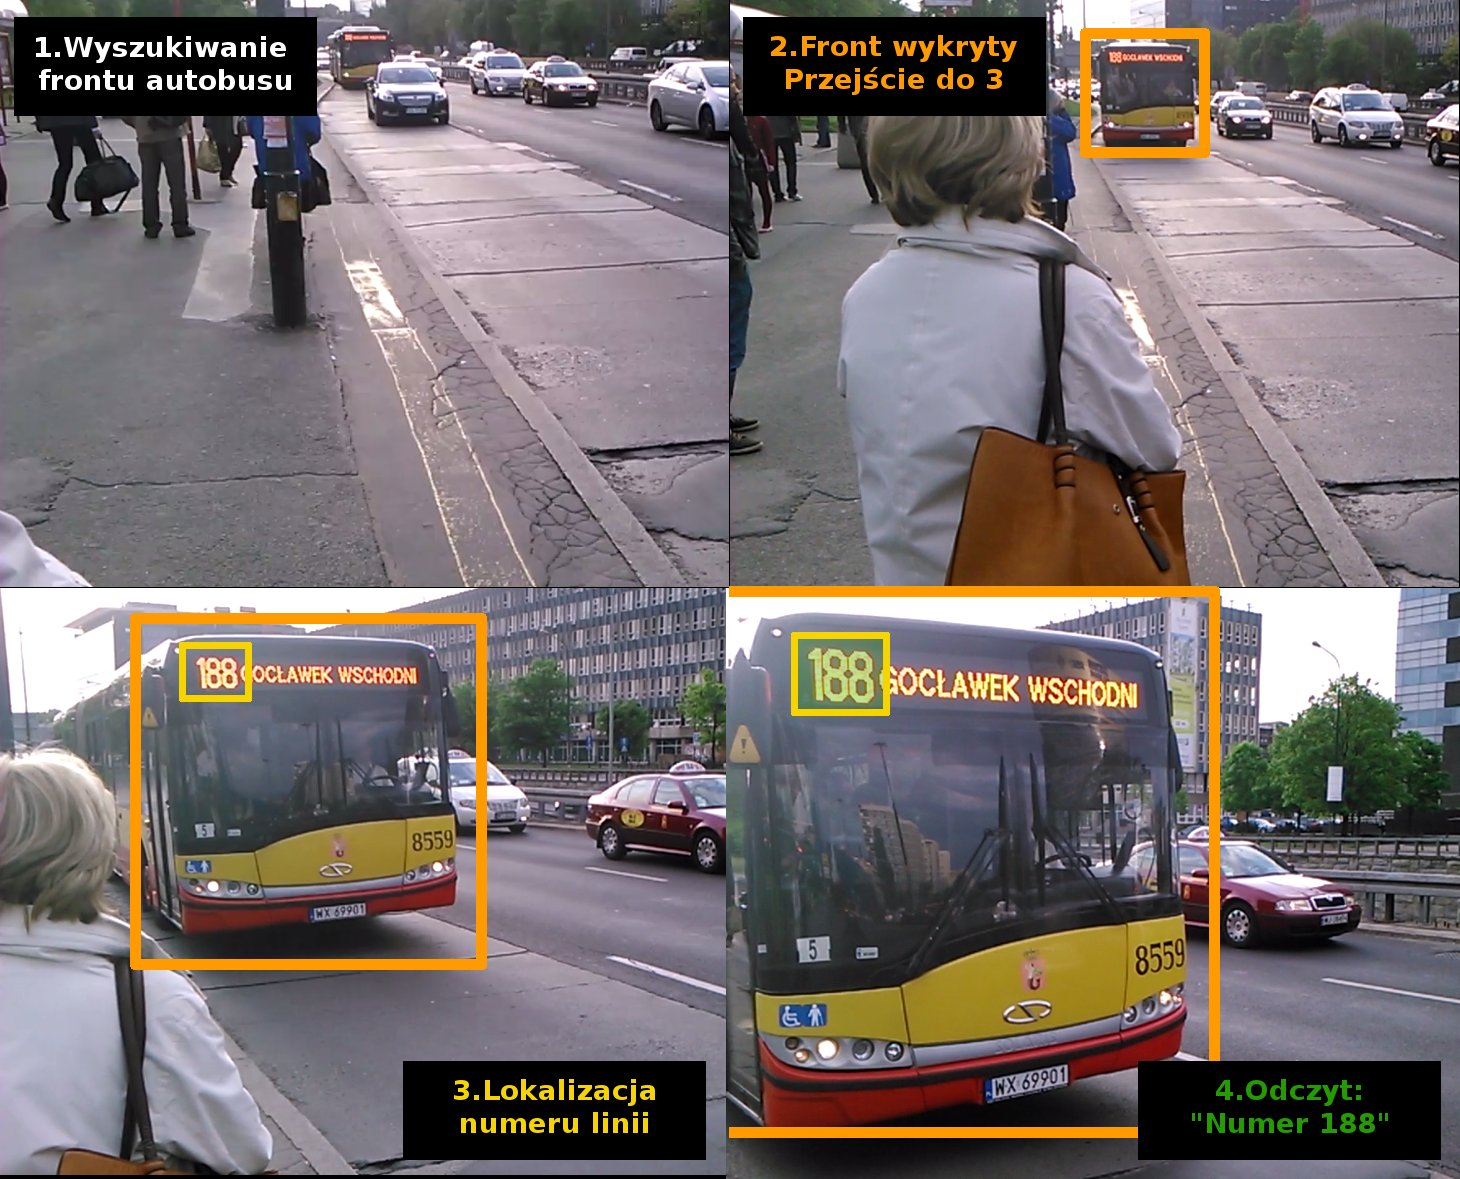
\includegraphics[width=0.9\textwidth]{img/int_use_case_sequence}
    \caption{Diagram przedstawiający przypadek użycia proponowanej aplikacji}
    \label{fig:int_use_case_diag}
\end{figure}

Elementem dodatkowym, nadającym sens całemu rozwiązaniu w~kontekście
wykorzystania aplikacji przez osoby niewidome i~niedowidzące,
byłoby wykorzystanie syntezatora tekstu na mowę dla 
odczytanego przez algorytm ciągu znaków reprezentującego numer linii. 
Scenariusz wykorzystania aplikacji zaprezentowano na rysunku
\ref{fig:int_use_case_diag}.


\section{Zakres pracy}

W~pracy zawarto przegląd dostępnych implementacji związanych
z~detekcją i~identyfikacją obiektów. W~drugim rozdziale 
wprowadzono obowiązujące
w~tym opracowaniu definicje detekcji i~identyfikacji. 
W~pierwszym podrozdziale omówiono metody wykrywania obiektów.
Skupiono się
głównie na istniejących rozwiązaniach, algorytmach, narzędziach 
i~bibliotekach. Duży nacisk położono na bibliotekę OpenCV. 
Jest ona bowiem dostępna na komputery PC, systemy Windows oraz Linux, 
urządzenia
mobilne, a~także system Android. Zaskakująco dobre
rezultaty skłoniły do opisania biblioteki OpenTLD. 
Drugi podrozdział to krótka wzmianka o~metodach
rozróżniania obiektów.

W~trzecim rozdziale przedstawiono proces implementacji
narzędzi wykorzystanych do zbudowania środowiska deweloperskiego
oraz testowego.

Kolejny - czwarty rozdział - opisywał wykonane doświadczenia.
W~pierwszej kolejności zamieszczono opis 
prób wykonanych w~celu identyfikacji najodpowiedniejszych 
narzędzi. Metody testowane 
w~tym rozdziale nie zostały wykorzystane w~rozwiązaniu końcowym.
W~podsumowaniu rozdziału czwartego zamieszczono opis prób kompletnej
implementacji, uruchamianej jednak jeszcze na komputerze stacjonarnym.

Piąty powstał w~wyniku implementacji rozwiązania na 
systemie docelowym. Opisano pierwsze próby aplikacji deweloperskiej
uruchomionej na dwóch podobnej klasy urządzeniach. Na końcu
zaprezentowano wyniki doświadczeń z~aplikacją demonstracyjną,
która zawierała już niemal całą zakładaną funkcjonalność.

Po implementacji programu na telefonie utworzone zostały zbiory 
i~narzędzia testowe. Opis uzyskanych w~ten sposób wyników, oraz
usprawnień końcowego systmu umieszczono na końcu rozdziału czwartego.
